\documentclass[11pt,a4paper]{article}
\usepackage[top=3cm, bottom=2cm, left=2cm, right=2cm]{geometry}
\usepackage[utf8]{inputenc}
\usepackage{amsmath, amsfonts, amssymb}
\usepackage{siunitx}
\usepackage[brazil]{babel}
\usepackage{graphicx}
\usepackage[margin=10pt,font={small, it},labelfont=bf, textfont=it]{caption}
\usepackage[dvipsnames, svgnames]{xcolor}
\DeclareCaptionFont{MediumOrchid}{\color[svgnames]{MediumOrchid}}
\usepackage[pdftex]{hyperref}
\usepackage{natbib}
\bibliographystyle{plainnat}
\bibpunct{\textcolor{MediumOrchid}{\textbf{[}}}{\textcolor{MediumOrchid}{\textbf{]}}}{,}{s}{}{}
\usepackage{color}
\usepackage{footnote}
\usepackage{setspace}
\usepackage{booktabs}
\usepackage{multirow}
\usepackage{subfigure}
\usepackage{fancyhdr}
\usepackage{leading}
\usepackage{indentfirst}
\usepackage{wrapfig}
\usepackage{mdframed}
\usepackage{etoolbox}
\usepackage[version=4]{mhchem}
\usepackage{enumitem}
\usepackage{caption}
\usepackage{titlesec}
\usepackage{tcolorbox}
\usepackage{tikz}
\usepackage{LobsterTwo}
\usepackage[T1]{fontenc}
\usepackage{fontspec}
\usepackage{txfonts}
\usepackage[bottom]{footmisc}

\makeatletter
\def\footnoterule{\kern-3pt\color{MediumOrchid}\hrule\@width0.6\textwidth height 0.8pt\kern2.6pt}
\makeatother

\renewcommand{\footnotelayout}{\itshape\color{MediumOrchid}}

\AtBeginEnvironment{equation}{\fontsize{13}{16}\selectfont}


\titleformat{\section}{\LobsterTwo\LARGE\color{CarnationPink}}{\thesection.}{1em}{}
\titleformat{\subsection}{\LobsterTwo\LARGE\color{CarnationPink}}{\thesubsection}{1em}{}


\DeclareCaptionLabelFormat{figuras}{\textcolor{DarkTurquoise}{Figura \arabic{figure}}}
\captionsetup[figure]{labelformat=figuras}

\makeatletter
\renewcommand\tagform@[1]{\maketag@@@{\color{CarnationPink}(#1)}}
\makeatother

\renewcommand{\theequation}{Eq. \arabic{equation}}
\renewcommand{\thefigure}{Fig. \arabic{figure}}
\renewcommand{\thesection}{\textcolor{CarnationPink}{\arabic{section}}}

\setlist[itemize]{label=\textcolor{CarnationPink}{$\blacksquare$}}

\setlist[enumerate]{label=\textcolor{CarnationPink}{\arabic*.}, align=left, leftmargin=1.5cm}


\newcounter{exemplo}

\NewDocumentEnvironment{exemplo}{ O{} }{%
\allowbreak
\setlength{\parindent}{0pt}
  \begin{mdframed}[
  leftline=true,
  topline=false,
  rightline=false,
  bottomline=false,
  linewidth=2pt,
  linecolor=CarnationPink,
  frametitlerule=false,
  frametitlefont=\LobsterTwo\large\color{CarnationPink},
  frametitle={\color{CarnationPink}\LobsterTwo\large #1},
  ]
}{%
  \end{mdframed}
}

\setlength{\fboxsep}{5pt}
\setlength{\fboxrule}{1.5pt}
\usepackage{float}
\renewcommand{\thefootnote}{\alph{footnote}}
\usepackage{url}
\hypersetup{
	colorlinks=true,
	linkcolor=DarkTurquoise,
	filecolor=DarkTurquoise,      
	urlcolor=DarkTurquoise,
	citecolor=DarkTurquoise,
	pdftitle={Especialista em Física da Radioterapia}
}
\pagestyle{fancy}
\fancyhf{}
\renewcommand{\headrulewidth}{0pt}
\rfoot{Página \thepage}

\title{\LobsterTwo\Huge{Radioterapia}}
\author{\LobsterTwo\Large{Aspectos Clínicos da Técnica de IGRT}\nocite{*}}
\date{\LobsterTwo\textit{Dalila Mendonça}}
\begin{document}
	\maketitle

\section{Introdução}

	A radioterapia guiada por imagem (IGRT) está bem estabelecida e existem várias estudos retrospectivos que avaliam o impacto do IGRT. O impacto potencial do IGRT pode ser apreciado considerando um estudo que relacionou falhas bioquímicas em pacientes com câncer de próstata à localização incorreta do alvo causada pela distensão retal no momento da simulação onde este problema pode ser corrigido com IGRT.

	A IGRT torna-se crucial quando se considera tratamentos de alta dose por fração, cujo exemplo mais extremo é a \textit{``Stereotactic Body Radiation Therapy''} (SBRT). O white paper da American Society for Radiation Oncology (ASTRO) \textbf{\textit{``Quality and Safety Considerations in Stereotactic Radiosurgery (SRS) and SBRT''}} observa que a orientação por imagem é “um pré-requisito para todas as aplicações SBRT”.

	O IGRT também é importante quando doses mais baixas e não ablativas são usadas, por exemplo, no tratamento hipofracionado do câncer de próstata em estágio inicial, que foi buscado com base na biologia vantajosa de uma baixa razão $\alpha/\beta$ em ensaios iniciais e depois em ensaios de grupo cooperativo (por exemplo, Radiation Therapy Oncology Group (RTOG) 0938).

\section{Revisão das Definições e Procedimentos de IGRT}

	A radioterapia guiada por imagem pode ser de vários tipos, conforme definido na Comissão Eletrotécnica Internacional (IEC) e também no TG-104 daAmerican Association of Physicists in Medicine:

	\begin{itemize}
		\item Correção “online” (ou seja, imediatamente antes ou durante a sessão de radioterapia e requer ajustes iniciados pelo operador);
		\item Correção “off-line” (ou seja, correção a ser aplicada na administração subsequente do tratamento -- próxima fração);
		\item O IGRT “em tempo real” é semelhante ao online, mas significa a aquisição de imagens durante o tratamento, permitindo o ajuste automático sem a intervenção de um operador.
	\end{itemize}

	O tipo de orientação por imagem depende das necessidades clínicas. Na SBRT, por exemplo, o white paper da ASTRO sobre segurança estereotáxica exige que a orientação por imagem seja aplicada "idealmente... no início de cada fração de tratamento", ou seja, online. As correções offline são valiosas para reduzir erros sistemáticos, mas não abordam variações aleatórias do dia a dia.
	
	Embora as correções on-line possam reduzir bastante as variações aleatórias, elas vêm com o custo da complexidade técnica. Os sistemas online de TC normalmente requerem 2 a 3 minutos extras para aquisição de imagem mais o tempo para interpretação. Eles também entregam dose extra, que merece consideração. O AAPM TG-75, \textbf{\textit{``The Management of Imaging Dose During IGRT''}}, observa que “o gerenciamento da dose da imagem durante a radioterapia é um problema diferente do gerenciamento da dose da imagem durante as imagens de diagnóstico de rotina ou procedimentos cirúrgicos guiados por imagem”. Embora este aplicativo possa não exigir um programa de radiologia diagnóstica como Image Gently (\href{http://www.pedrad.org/associations/5364/ig/}{http://www.pedrad.org/associations/5364/ig/}) ou Image Wisely (\href{http://www.imagewisely.org/}{http://www.imagewisely.org/}), claramente um é necessária uma consideração equilibrada de custo/benefício. O relatório observa que “não é mais seguro \dots presumir que a dose cumulativa da imagem é insignificante em comparação com a dose terapêutica”.

	Há uma grande variedade de tecnologias para realizar os vários tipos de IGRT, conforme descrito na \ref{fig:tiposdeIGRT}. É importante observar que, com a possível exceção das tecnologias de RM durante o tratamento, nenhuma plataforma pode atingir todas as metas clínicas do IGRT.

	\begin{figure}[h]
		\centering
		\fcolorbox{DarkTurquoise}{white}{%
			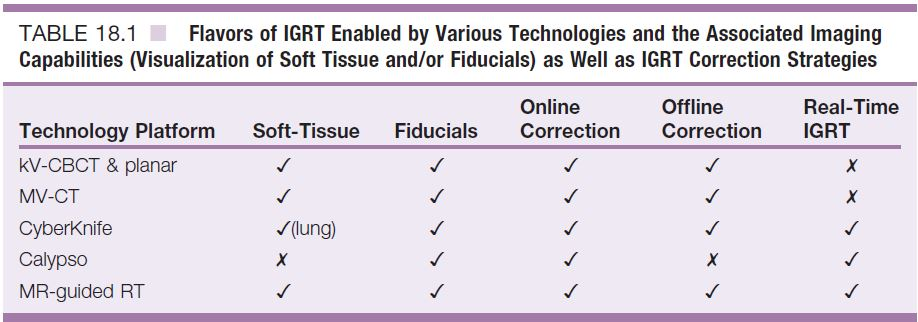
\includegraphics[width=0.8\textwidth]{Imagens/tiposdeIGRT.JPG}
		}%
		\caption{Tipos de IGRT habilitados por várias tecnologias e recursos de imagem associados (visualização de tecidos moles e/ou fiduciais), bem como estratégias de correção de IGRT.}
		\label{fig:tiposdeIGRT}
	\end{figure}

\subsection{Exemplo de Fluxo Utilizando IGRT baseada em CT}

	Um primeiro passo no IGRT e um fundamento chave é a imagem de referência usada para o planejamento do tratamento (neste caso, a CT de simulação, \ref{cbctIgrt}\textcolor{DarkTurquoise}{A}). Um isocentro e conjuntos de estruturas de região de interesse são definidos no sistema de planejamento de tratamento. Estes são transferidos (se necessário) para o sistema de orientação por imagem. Quando o paciente está pronto para o tratamento e posicionado no isocentro pretendido, uma TC é adquirida (\ref{cbctIgrt}\textcolor{DarkTurquoise}{B}). Essa TC é alinhada com o conjunto de dados de referência usando uma interface de software de fusão de imagem interativa (\ref{cbctIgrt}\textcolor{DarkTurquoise}{C}).
	\begin{figure}[!h]
		\centering
		\subfigure{
			\fcolorbox{DarkTurquoise}{white}{%
				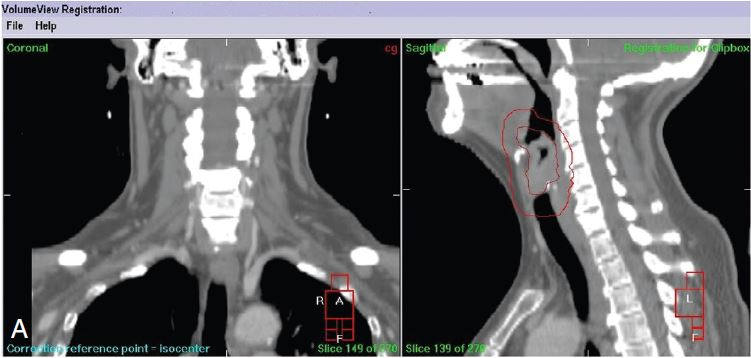
\includegraphics[width=0.6\textwidth]{Imagens/cbcta.JPG}
			}} \\
		\subfigure{
			\fcolorbox{DarkTurquoise}{white}{%
				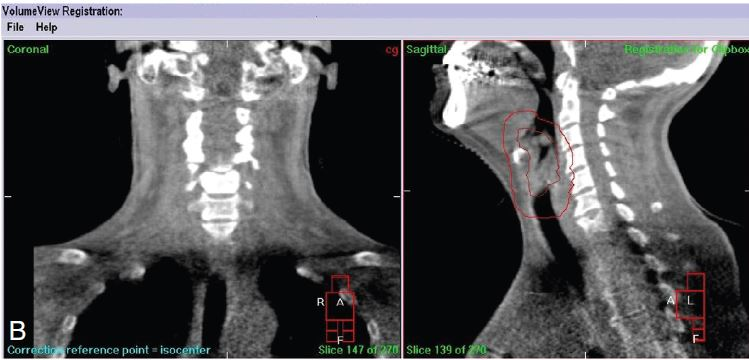
\includegraphics[width=0.6\textwidth]{Imagens/CBCTB.JPG}
			}} \\ %
		\subfigure{
			\fcolorbox{DarkTurquoise}{white}{%
				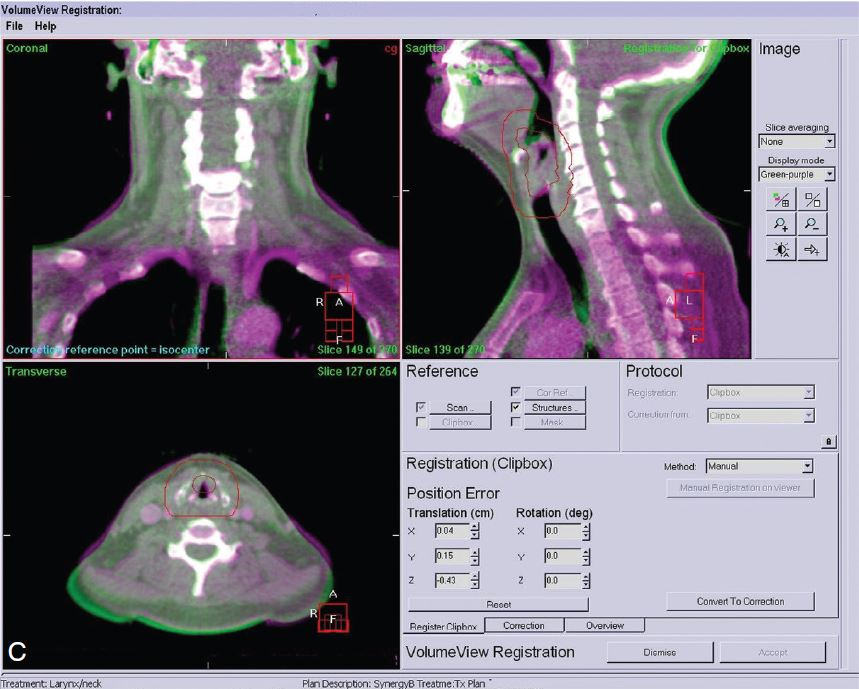
\includegraphics[width=0.6\textwidth]{Imagens/cbctc.JPG}
		}} \\ %	
		\caption{Alinhamento baseado em TC de feixe cônico (CBCT) de um paciente em tratamento de câncer de cabeça e pescoço. Antes do tratamento, uma varredura de CBCT é adquirida (B) e fundida com a TC de referência da simulação (A). Observe que algumas regiões se alinham bem, mas outras não (C).}
		\label{fig:cbctIgrt}
	\end{figure}

	O registro usa o alinhamento de corpo rígido com translações 3D e,opcionalmente, rotações em torno de três eixos. O registro pode ser realizado manualmente ou automaticamente por meio de vários algoritmos que podem ser configurados para focar em regiões específicas da imagem (por exemplo, uma caixa 3D) oou em diferentes valores de limiar do número CT (por exemplo, características ósseas ou tons de cinza de tecido mole). O registro resulta em um valor calculado de correção de deslocamento. O paciente é movido de acordo com esses cálculos de deslocamento, onde esse processo geralmente é realizado automaticamente por meio de um comando para a mesa do linac. 

	Alguns sistemas de suporte ao paciente (por exemplo, HexaPod) permitem a correção do posicionamento de “seis graus de liberdade” (ou seja, movimentos translacionais em três direções, bem como rotações de até 3 graus sobre os três eixos principais). Um problema é que a rotação pode descrever corretamente o alinhamento anatômico perto do isocentro, mas pode ser menos precisa longe do isocentro. Uma rotação de 1 grau corresponde a um deslocamento de aproximadamente 2 mm a 10 cm do isocentro. Esses alinhamentos imprecisos fora do isocentro podem ter implicações para doses em órgãos de risco.

	Seja qual for a estratégia de correção, é importante ter um protocolo pré-definido para o IGRT que inclua as funções e as responsabilidades de cada grupo profissional e os protocolos associados. Um exemplo de protocolo de um hospital fictício é apresentado na Tabela 18.2. O protocolo especifica quem é o responsável pelo alinhamento do IGRT (técnicos de radioterapia neste caso). Este exemplo também lista os limites para deslocamentos (10 mm), acima dos quais eles devem consultar um radio-oncologista. Esses limites são uma recomendação específica dos guidelines da ACR/ASTRO para IGRT e, idealmente, devem ser específicos para a instituição e baseados em uma análise dos erros aleatórios e sistemáticos. O protocolo de exemplo também especifica as funções profissionais. Aqui, espera-se que o médico e o físico estejam presentes para o procedimento de alinhamento no primeiro dia, mas não depois disso. Isso pode variar para outros protocolos de tratamento. Nos casos de SBRT, por exemplo, o médico normalmente estaria presente em cada fração do tratamento.

	A este processo IGRT idealizado são adicionados os muitos problemas e desafios que podem surgir na prática real. Um caminho de erro bem usado está relacionado ao posicionamento do isocentro. O sistema de orientação por imagem deve ter o ponto de referência correto definido, geralmente o isocentro de planejamento de tratamento definido no TPS. Se um ponto de referência incorreto for transferido, o alinhamento do paciente ficará incorreto. Este erro é particularmente insidioso porque não é visível para o operador. Da mesma forma, em um sistema TomoTherapy, a referência ou os lasers vermelhos devem ser definidos para o ponto de referência no sistema de planejamento. Não fazer isso levará a erros sistemáticos.

	Outros erros menos grosseiros são possíveis. Por exemplo, o preenchimento da bexiga para um caso de pelve pode ser diferente no momento do tratamento em comparação com a simulação. Em tal situação, não seria possível alinhar toda a anatomia pélvica sem intervenção do paciente e fazer uma nova aquisição de imagem. A \ref{cbctIgrt}\textcolor{DarkTurquoise}{B} mostra um exemplo de um paciente com câncer de cabeça e pescoço em que parte da anatomia está bem alinhada (vértebras cervicais), mas outra parte não está (mandíbula e crânio). Tais erros de alinhamento da região representam um desafio significativo quando extensas regiões estão sendo tratadas e ressaltam a importância do envolvimento do médico na definição dos objetivos de alinhamento para casos de IGRT. 

	Outra questão é quão bem a tomografia computadorizada de planejamento (adquirida antes do tratamento) representa a anatomia durante o tratamento real. Vários problemas estão relacionados a aquisição da tomografia de planejamento prévia: movimento do paciente, imobilização não ideal, longos tempos de espera entre o exame e o tratamento, mudanças no tamanho ou posição do tumor durante o tratamento e mudanças no habitus corporal do paciente (por exemplo, perda de peso). Para avaliar o movimento em casos individuais, pode ser útil repetir a TC logo após o tratamento para avaliar se houve movimento (talvez para várias frações). Para tratamentos mais demorados (por exemplo, SRS/SBRT), podem ser realizadas outras imagens no meio da entrega do tratamento. 

\subsection{Exemplo de Fluxo Utilizando IGRT em Tempo Real}

	Cenários de fluxo de tratamento para IGRT em tempo real compartilham muitas semelhanças com a discussão anterior sobre IGRT baseado em CT. Os detalhes dependem da tecnologia, mas um exemplo simples são as imagens planares em um sistema realizado em um linac. Novamente, uma imagem de referência (radiografia reconstruída digitalmente (DRR)) é necessária. 

	Os sistemas IGRT modernos permitem sobrepor ou fundir a DRR com a imagem online e também desenhar regiões no DRR (por exemplo, um ponto de referência ósseo ou fiducial implantado), que são então sobrepostos com a imagem online. As imagens online podem ser imagens de dispositivo eletrônico de imagem de portal (EPID) de megavoltagem (MV), mas a imagem planar kV normalmente resulta em melhor qualidade de imagem e doses mais baixas (\ref{fig:protocoloImagemPlanar}). No exemplo da \ref{fig:protocoloImagemPlanar}\textcolor{DarkTurquoise}{B}, o alinhamento dos clipes cirúrgicos está sendo monitorado durante o tratamento.

	\begin{figure}[!h]
		\centering
		\fcolorbox{DarkTurquoise}{white}{%
			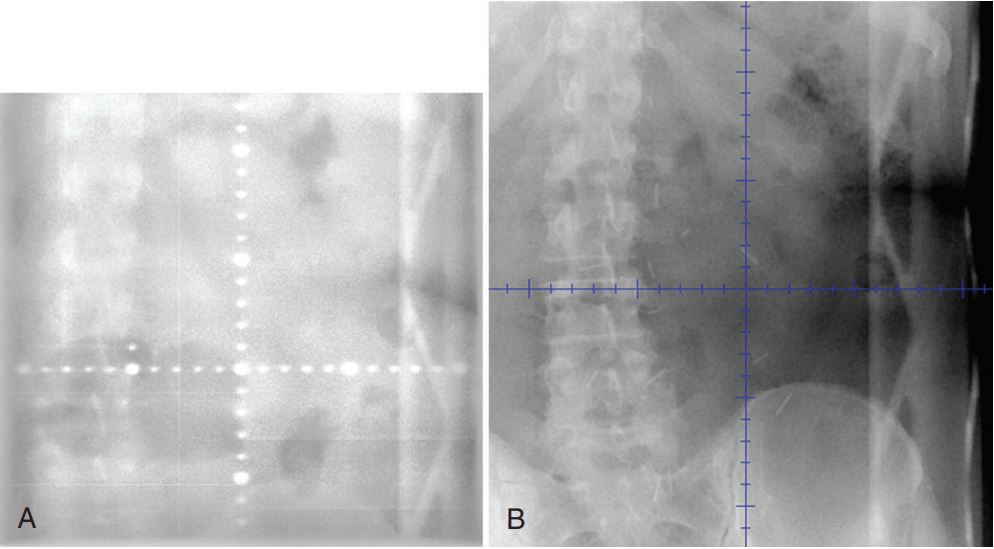
\includegraphics[width=0.8\textwidth]{Imagens/protocoloImagemPlanar.JPG}
		}%
		\caption{Imagens planares adquiridas para alinhamento usando o (A) feixe MV e (B) o feixe kV .}
		\label{fig:protocoloImagemPlanar}
	\end{figure}

	Outro exemplo de orientação em tempo real é o uso de sinalizadores (beacon) de radiofrequência implantados, atualmente aprovados para uso na próstata. Cada sinalizador é identificado na tomografia de referência e tem uma frequência única. As posições dos sinalizadores são então monitoradas em tempo real durante o tratamento. Quando a orientação por imagem em tempo real é utilizada, níveis de ação devem ser estabelecidos para a interrupção do tratamento. No cenário do movimento respiratório, esses níveis de ação podem depender do método utilizado para a compensação respiratória.

\section{Protocolos de Imagens}

	Existem vários parâmetros que controlam a aquisição da imagem. Uma configuração importante para a TC é a extensão da anatomia visualizada, que pode ser controlada pela colimação, conforme mostra a \ref{fig:parametrosIgrtTc}.

	\begin{figure}[h]
		\centering
		\fcolorbox{DarkTurquoise}{white}{%
			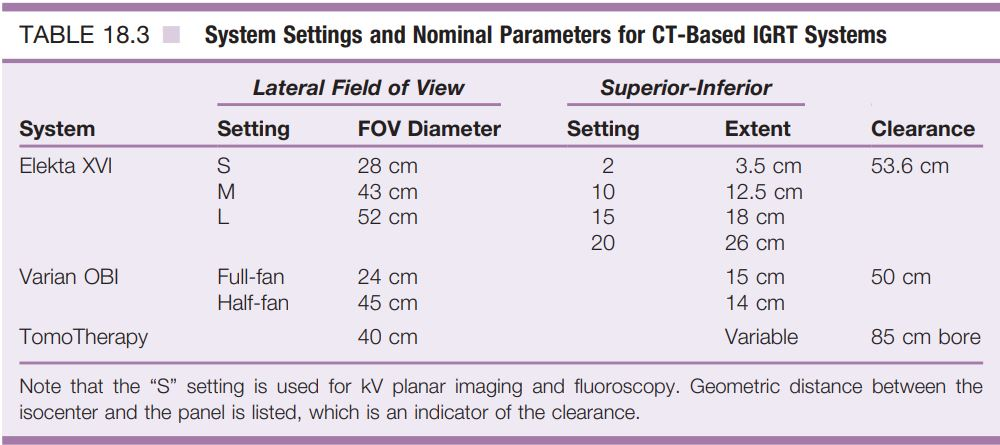
\includegraphics[width=0.8\textwidth]{Imagens/parametrosIgrtTc.JPG}
		}%
		\caption{Configurações do sistema e parâmetros nominais para sistemas IGRT baseados em TC.}
		\label{fig:parametrosIgrtTc}
	\end{figure}

	As configurações podem ser usadas em várias combinações com compensações associadas entre a qualidade da imagem e a extensão da anatomia visível. Uma configuração grande (por exemplo, L20 ou meio-leque --\ref{fig:parametrosIgrtTc}) produz uma anatomia extensa, talvez até mesmo o contorno externo do paciente. No entanto, em comparação com uma configuração menor (por exemplo, S10 ou leque-completo) a aquisição maior resultará em um aumento do ruído devido ao aumento no espalhamento e aos artefatos de cupping.  Além disso, o paciente é exposto a uma quantidade maior de radiação.

	O número de projeção de imagens adquiridas também é controlável. Em um sistema (Elekta Inc.), a aquisição pode ser feita a partir de uma rotação inteira do gantry (“full-scan”) ou pode ser limitada a uma rotação de \ang{200} (“half-scan”). Uma half-scan é mais rápida (70 segundos versus 1.5 minutos), mas está sujeita a streaks em cortes axiais. 

	O tamanho dos voxels usados na reconstrução também pode ser controlado. Este sistema da Elekta usa voxels isotrópicos (resolução baixa: 2 mm, resolução média: 1 mm e resolução alta: 0.5 mm) com slice médio selecionável na dimensão longitudinal. O sistema On-Board Imaging (OBI) da Varian usa outros protocolos (leque-completo: 0.47 x 0.47 x 2.5 mm ou meio-leque: 0.88 x 0.88 x 2.5 mm). O TomoTherapy usa valores de pitch pré-programados de 1, 2 e 3 (fino, normal e grosseiro) com um colimador de 4 mm (ou seja, espessuras nominais dos slices de 2, 4 e 6 mm). Conforme revisado no AAPM TG-148, o período de rotação do TomoTherapy durante a aquisição da imagem é fixado em 10 segundos, o que se traduz em uma taxa de aquisição de um corte a cada 5 segundos para uma técnica de reconstrução half-scan. O campo de visão axial (field of view - FOV) é definido em 40 cm com um tamanho de voxel de 0.78 mm. A extensão superior-inferior depende de quantos cortes são adquiridos. 

	Além dessas considerações técnicas, a qualidade da imagem e a orientação são afetadas de maneiras mais complexas por várias situações clínicas. A \ref{cbctIgrt}\textcolor{DarkTurquoise}{B} mostra uma aquisição de CBCT em que a qualidade da imagem é boa em uma região (a área mais fina da cabeça e do pescoço), mas pior em outra região (a região mais espessa perto dos ombros). Em alguns casos, isso é aceitável, mas em outros casos a técnica precisaria ser modificada (por exemplo, configurações de mAs mais altas, kVp mais alto ou uso da técnica de full-scan em vez de  half-scan).

	Outro problema que afeta a qualidade da imagem é o movimento do paciente, que é comum devido aos longos tempos de aquisição da varredura ($>$ 1 minuto). O movimento resulta em borramento, o que às vezes é difícil de avaliar. O movimento respiratório é um caso especial disso. Novos desenvolvimentos permitem CBCT 4D por meio do qual o movimento respiratório pode ser visualizado, embora com um longo tempo de aquisição (3 a 4 minutos). Se um paciente estiver sendo tratado com gerenciamento de movimento respiratório (por exemplo, gating ou breath hold), então a CBCT deve ser adquirida com esse gerenciamento em vigor. Nesse caso, o movimento é mínimo, mas os tempos de varredura podem ser longos (por exemplo, cinco ou mais aquisições em breath-hold para uma única TC).

\section{Mudanças Anatômicas e Radioterapia Adaptativa}

	As alterações anatômicas representam uma das principais vantagens do IGRT e também um dos desafios mais significativos. Do lado positivo, o IGRT permite corrigir alterações sistemáticas no tratamento versus no momento da simulação. O estudo de 2005 de \citet{de2005increased}  do MD Anderson descobriu que o aumento do enchimento retal no momento da simulação resultou em aumento da falha bioquímica. Acredita-se que isso se deva ao deslocamento posterior sistemático da próstata durante o tratamento em relação ao plano de tratamento. O IGRT oferece uma oportunidade para corrigir isso.

	Alterações anatômicas também podem apresentar desafios significativos para o IGRT. Uma situação particularmente difícil são as mudanças durante o tratamento em pacientes com câncer de pulmão de não-pequenas células submetidos ao tratamento padrão (por exemplo, 60 Gy administrados em 33 frações). Alguns desses tumores irão diminuir durante o tratamento para menos da metade do tamanho original. Se o centróide do tumor for alinhado a cada dia, a anatomia ao redor estará bastante deslocada ao final do tratamento. Além disso, a redução é muitas vezes direcionalmente assimétrica. O alinhamento pode ser ainda mais complicado pela resolução da atelectasia durante o tratamento. Para reduzir o impacto desses efeitos, alguns médicos re-simulam e replanejam esses pacientes no meio do tratamento.

	A radioterapoa adaptativa (ART) é uma abordagem para lidar com as mudanças anatômicas durante o tratamento. O conceito básico é reotimizar o plano do paciente usando uma tomografia computadorizada adquirida no momento do tratamento. Isso pode ser feito online, com planejamento rápido, ou offline, com um novo planejamento desenvolvido para ser aplicado no dia seguinte. Até 2010, apenas um sistema de ART fornecido por um fabricante estava aprovado pela Food and Drug Administration (FDA), sendo ele um sistema baseado em ressonância magnética da ViewRay Inc. 

	Ainda não existem recomendações a nível de grupo de trabalho sobre o uso da Radioterapia Adaptativa (ART), embora seja claramente necessário orientações devido às importantes considerações de fluxo de trabalho, entrega e segurança. No entanto, há uma extensa quantidade de literatura sobre esse tema (consulte Ghilezan et al., por exemplo, para uma revisão sobre câncer de próstata). Pelo menos um ensaio prospectivo utilizando a ART foi publicado. Na ausência de ferramentas comerciais amplamente disponíveis, algumas clínicas estão empregando a ART "manualmente", realizando replanejamentos de pacientes em casos com mudanças anatômicas suficientemente grandes para terem um impacto dosimétrico clinicamente significativo, conforme avaliado pelo médico. No entanto, é importante ressaltar que a construção de uma distribuição de dose composta diante de mudanças anatômicas é, no melhor dos casos, aproximada. Pode não ser possível recalcular a dose, sendo necessário deformar a dose dentro do sistema, caso a recálculo não seja viável. Esse processo não leva em conta alterações na densidade ou contornos externos. Mesmo em sistemas completamente capazes de ART, pode haver situações em que a dose não possa ser recalculada (por exemplo, em CT online truncada). 


\section{Gerenciamento de Um Programa IGRT}

	Para garantir a segurança e eficácia de um programa de IGRT, não é suficiente apenas ter recursos técnicos e clínicos adequados. Aspectos organizacionais e de gestão desempenham um papel crucial. O white paper da ASTRO identificou dez elementos fundamentais que devem ser considerados para uma boa prática de IGRT.

	\begin{enumerate}
		\item  formação de uma equipe multiprofissional responsável pelas atividades de IGRT
		\item o estabelecimento de programas de garantia da qualidade diários, mensais e anuais
		\item o fornecimento de treinamento específico para toda a equipe envolvida na operação e entrega de IGR. A IGRT requer um conjunto de habilidades além das tradicionalmente exigidas. Por exemplo, os técnicos em radioterapia requerem expertise em anatomia seccional e leitura de imagens de ultrassom.
		\item Realizar testes "ponta a ponta" para todos os novos procedimentos de IGRT.
		\item Estabelecer documentação e procedimentos específicos para a IGRT.
		\item Identificar claramente quem é responsável pela aprovação das decisões de correção de IGRT e o processo pelo qual essas decisões são tomadas e documentadas.
		\item Estabelecer e documentar procedimentos de planejamento específicos para cada local, incluindo o procedimento para definição de margens de volume alvo de planejamento (PTV).
		\item Realizar revisão por pares multiprofissional dos volumes de PTV e revisão por pares dos volumes de volume tumoral bruto/volume alvo clínico (GTV/CTV) por radioterapeutas.
		\item Verificar a criação correta e transferência de dados de referência de IGRT (PTV, OARs, DRRs, etc.) para o sistema de IGRT.
		\item Estabelecer um mecanismo de relato para variações relacionadas à IGRT no processo de tratamento radioterápico.
	\end{enumerate}
	
	Esses elementos visam garantir a consistência, qualidade e segurança do programa de IGRT como um todo.

\section{Aplicações de IGRT}

\subsection*{Próstata}

	Os gradientes de dose acentuados utilizados na borda posterior da próstata são necessários para minimizar a exposição à radiação de tecidos saudáveis próximos, como o reto e a bexiga e, portanto, tornam a Radioterapia Guiada por Imagem (IGRT) particularmente útil, especialmente porque permite ir além da anatomia óssea e localizar a própria glândula prostática, bem como permite a visualização do preenchimento retal e da bexiga quando se utiliza imagens volumétricas.. Diversas tecnologias têm sido utilizadas: ultrassom (AAPM TG-154), tomografia computadorizada (TC) durante o tratamento e marcadores implantados ou beacons de radiofrequência (Calypso Inc.). Acredita-se que no futuro próximo, a radioterapia guiada por ressonância magnética também será utilizada para o tratamento da próstata, oferecendo ainda mais precisão e visualização do alvo e dos órgãos circundantes durante o processo de tratamento.

	Durante o tratamento de radioterapia guiada por imagem (IGRT) para a próstata, a complexidade das estruturas-alvo pode ser um desafio adicional. Em casos em que o tratamento é realizado em várias fases, como quando se inclui as vesículas seminais e/ou gânglios regionais, nem todas as regiões anatômicas podem ser alinhadas simultaneamente. Nesses casos, quando a radioterapia adaptativa não está disponível ou quando não foram criados conjuntos de planos antecipadamente, uma estratégia comum é o alinhamento com base na anatomia óssea. Já na fase de reforço ou "redução do campo", o foco do alinhamento se concentra na próstata em si, com atenção especial às interfaces próstata/bexiga/reto. No entanto, mesmo nesse caso, a glândula prostática pode sofrer rotações de inclinação (pitch), principalmente quando há mudanças no preenchimento da bexiga ou do reto. Essas rotações podem não ser completamente corrigidas mesmo com o uso de sistemas de posicionamento de pacientes com seis graus de liberdade (normalmente limitados a uma rotação inferior a 3 graus). Alguns grupos de pesquisa têm observado variações significativas no volume retal entre as sessões de tratamento, o que levou à defesa do planejamento e tratamento com o reto vazio, sendo uma abordagem que parece reduzir essa variabilidade e melhorar a precisão do tratamento.

	Durante o tratamento de radioterapia da próstata, o movimento da próstata é uma preocupação devido à peristalse (contração rítmica do intestino) e ao relaxamento dos músculos pélvicos. Ao longo do tratamento, a próstata pode sofrer um deslocamento lento para trás. Para lidar com esse desafio, são utilizadas técnicas de imagem em tempo real, como marcadores implantados ou beacons de radiofrequência (Calypso Inc.). Esses dispositivos permitem acompanhar a posição da próstata durante o tratamento em tempo real. No entanto, a utilização dessas técnicas também apresenta desafios próprios. No passado, havia preocupações quanto à migração dos marcadores dentro do tecido prostático, mas estudos demonstraram que esse não é um problema significativo. No entanto, é essencial implantar os marcadores com precisão para garantir uma localização adequada. Geralmente, três marcadores são implantados, mas é importante que eles estejam espaçados corretamente para evitar uma redução na precisão da localização tridimensional. É importante ressaltar que essas questões são particularmente relevantes para sistemas que não dependem de imagens volumétricas, ou seja, para sistemas que não fornecem uma imagem completa do órgão-alvo em tempo real durante o tratamento.

	Quando se trata de utilizar a IGRT na próstata, é importante ter cuidado ao definir as margens de tratamento. Embora a IGRT forneça uma localização mais precisa do tumor, é necessário levar em consideração que pequenas variações na posição da próstata podem ocorrer durante o tratamento. Portanto, é comum utilizar margens de segurança em torno da próstata para garantir que toda a região do tumor seja abrangida pela radiação. No entanto, é crucial encontrar um equilíbrio adequado, pois margens muito estreitas podem resultar em uma cobertura insuficiente do tumor, levando a um aumento do risco de falha de tratamento. Em um estudo realizado em um centro europeu em 2009, foi observado que pacientes submetidos à IGRT baseada em marcadores apresentaram uma redução significativa na taxa de sucesso bioquímico. Esse resultado foi atribuído a uma redução excessivamente agressiva nas margens utilizadas no tratamento (3 mm na direção lateral, 4 mm na direção cranial-caudal e 5 mm na direção ântero-posterior), enquanto um valor de 6 mm poderia ter sido mais apropriado para abranger adequadamente o tumor e garantir melhores resultados. Portanto, é essencial ter uma abordagem cautelosa ao definir as margens de tratamento durante a IGRT, considerando tanto a precisão da localização do tumor quanto a necessidade de uma cobertura adequada para garantir o sucesso do tratamento.


\subsection*{Cabeça e Pescoço}

	A radioterapia da cabeça e pescoço (H\&N) é um cenário ideal para a IGRT pois apresenta desafios específicos devido à proximidade dos tumores com órgãos de risco, como a medula espinhal e a glândula parótida. Além disso, os planos de tratamento muitas vezes têm gradientes de dose acentuados, o que exige um alto nível de precisão na entrega da radiação. No entanto, a H\&N também apresenta desafios adicionais devido ao uso de campos de tratamento extensos para tratar doenças avançadas ou regiões de gânglios de risco no pescoço. Os grandes volumes tumorais combinados com a anatomia flexível do pescoço tornam o alinhamento da IGRT um desafio complexo. Alguns centros podem optar por utilizar uma técnica de alinhamento rígido, ignorando a deformação anatômica diária causada por movimentos não rígidos, como a flexão do pescoço e a posição da mandíbula. No entanto, estudos mostram que essa abordagem não é apropriada. Pesquisas iniciais utilizando imagens volumétricas para a H\&N alinharam uma parte específica da anatomia vertebral e mediram os erros residuais em outras partes, constatando a presença de erros residuais de 2 a 6 mm. Estudos mais recentes confirmaram esses achados e sugerem uma abordagem em que múltiplas regiões são alinhadas simultaneamente durante o tratamento. Isso ajuda a minimizar os erros de alinhamento e a garantir uma entrega de dose mais precisa e eficaz no tratamento da H\&N.

	Durante o tratamento de radioterapia da cabeça e pescoço, é comum observar uma significativa mudança no volume dos tecidos ao longo do tempo. Estudos iniciais relataram que os volumes tumorais (GTVs) tendem a diminuir em cerca de metade do tamanho inicial durante o tratamento. Além disso, os linfonodos e as glândulas parótidas também sofrem redução de tamanho e um deslocamento medial. Essas alterações são resultado da resolução do tumor, das mudanças pós-cirúrgicas e/ou da perda de peso do paciente. No entanto, se essas mudanças não forem consideradas e ajustes apropriados não forem feitos no plano de tratamento, pode ocorrer uma subdosagem significativa do tumor e uma superdosagem em estruturas normais. Para lidar com esse desafio, a solução mais promissora é a utilização da radioterapia adaptativa, que envolve o uso de técnicas avançadas de registro de imagem deformável. Essa abordagem permite que o plano de tratamento seja ajustado e adaptado ao longo do tempo, levando em consideração as mudanças anatômicas do paciente. Embora a radioterapia adaptativa ainda esteja em desenvolvimento, ela representa uma direção futura importante para melhorar a precisão e eficácia dos tratamentos de H\&N.

\subsection*{Pulmão}

	A IGRT de tumores pulmonares apresenta características únicas em comparação com outros locais de tratamento. No pulmão periférico, os tumores são bem visíveis, o que significa que podem ser facilmente identificados nas imagens de radiografia planar ou tomossíntese. Isso é uma vantagem em relação a outros locais de tratamento, como o fígado, onde os tumores geralmente são menos visíveis e podem requerer o uso de marcadores fiduciais para auxiliar na localização precisa. A capacidade de visualizar o tumor diretamente nas imagens radiográficas planares permite o alinhamento intrafração, ou seja, ajustes precisos da posição do paciente durante a própria sessão de tratamento. Essa abordagem é comumente usada em tratamentos com CyberKnife, mas também pode ser realizada em plataformas de aceleradores lineares. O alinhamento intrafração é uma estratégia importante para garantir a precisão na entrega da radiação e reduzir a dose em tecidos saudáveis adjacentes.

	No tratamento de radioterapia guiada por imagem (IGRT) no pulmão, um dos principais desafios é o movimento respiratório,como discutido no relatório da AAPM TG-76, "The Management of Respiratory Motion in Radiation Oncology", que pode afetar a precisão da entrega da radiação. Para lidar com esse desafio, são utilizadas várias técnicas e abordagens. A tomografia computadorizada 4D é uma ferramenta importante, pois permite medir e visualizar o movimento respiratório durante a simulação. Recentemente, a tomografia computadorizada 4D também se tornou disponível em algumas unidades de tratamento, o que é útil para confirmar o alinhamento e o movimento. Os dados 4D podem ser utilizados no planejamento do tratamento para gerar um volume-alvo interno (ITV), que leva em consideração a variabilidade do movimento respiratório. Além disso, os dados podem ser processados para gerar uma projeção de intensidade máxima (MIP), que mostra o valor máximo de pixels em todas as fases respiratórias, ou uma tomografia computadorizada média, que representa a média de cada pixel. Essas informações auxiliam no planejamento e no ajuste adequado do tratamento. Além disso, técnicas como a compressão torácica, o gating respiratório e a apneia respiratória podem ser utilizadas para controlar o movimento respiratório durante o tratamento. É importante garantir que as técnicas de IGRT utilizadas durante o tratamento sejam consistentes com as utilizadas durante a simulação, para garantir a precisão e a eficácia do tratamento.

	Durante o tratamento de radioterapia pulmonar com IGRT, é importante considerar as mudanças que ocorrem nos tumores e atelectasias ao longo do tempo. Estudos mostram que os volumes dos tumores de câncer de pulmão de não-pequenas células tendem a encolher cerca de 1\% por dia durante o tratamento. Além disso, esse encolhimento pode ocorrer de forma assimétrica, ou seja, diferentes partes do tumor podem encolher em taxas diferentes. Essas mudanças no tamanho e na forma do tumor podem afetar a precisão da entrega da radiação, pois os planos de tratamento são baseados nas características do tumor durante a simulação. Para contornar esse desafio, a radioterapia adaptativa é uma abordagem promissora. Ela envolve a realização de novas imagens de imagem durante o tratamento, como a tomografia computadorizada 4D, para avaliar o encolhimento do tumor e fazer ajustes no plano de tratamento. Dessa forma, é possível garantir que a dose de radiação seja adequadamente direcionada ao tumor, mesmo à medida que ele encolhe. A radioterapia adaptativa representa uma direção futura importante para melhorar a precisão e eficácia da IGRT pulmonar.

\section{Principais Tópicos}

	A IGRT desempenha um papel central na Radioterapia moderna, especialmente em tratamentos hipofracionados ou estereotáxicos. A IGRT pode aumentar a confiança de que os tratamentos estão direcionados ao local desejado e ajudar a reduzir as margens de volume de tratamento quando apropriado. A IGRT também é fundamental na técnica emergente da ART (Adaptive Radiation Therapy), que aborda as mudanças anatômicas durante o tratamento, reotimizando o plano do paciente com base em novas informações de imagem. Uma ampla variedade de tecnologias está disponível para a IGRT, com o objetivo de melhorar a precisão do tratamento por meio de uma ou mais das seguintes estratégias: correção online (imediatamente antes do tratamento), correção offline (aplicada antes da próxima fração) ou monitoramento em tempo real (durante o tratamento). Os benefícios da IGRT devem ser ponderados em relação às desvantagens potenciais. Os sistemas de TC online normalmente exigem de 2 a 3 minutos extras para aquisição de imagens, além do tempo de interpretação. Eles também fornecem uma dose extra, o que merece consideração e pode se tornar significativo se a IGRT for usada diariamente durante várias semanas de tratamento. No aspecto técnico, os protocolos de aquisição de IGRT podem ser controlados até certo ponto para otimizar as várias variáveis dependentes, como qualidade da imagem, tempo de escaneamento e extensão da anatomia visualizada. Esses fatores geralmente envolvem compensações entre si, e a orientação do médico é necessária para encontrar o protocolo de escaneamento ideal (ou seja, mais imagens adquiridas podem resultar em melhor resolução, mas levar mais tempo e fornecer uma dose maior ao paciente).

	Grandes volumes tumorais na cabeça e no pescoço, por exemplo, tornam o alinhamento da IGRT desafiador, especialmente devido à anatomia flexível do pescoço. No pulmão, um grande desafio é o movimento respiratório, e as técnicas de alinhamento devem levar isso em consideração. De forma mais geral, a dose nos tecidos normais às vezes pode ser maior com a IGRT, o que é um pouco contraditório. Um exemplo é o reto em um tratamento de câncer de próstata. Devido às variações diárias no posicionamento, o reto às vezes é posicionado em uma região de baixa dose. No entanto, se a IGRT for utilizada, o reto pode ser posicionado de forma mais consistente na região de alta dose em comparação com um caso em que a IGRT não é utilizada.

	A segurança e a eficácia de um programa de IGRT dependem, argumentavelmente, tanto dos aspectos organizacionais e de gestão quanto das características técnicas e clínicas. Diretrizes estão disponíveis em organizações profissionais para auxiliar nesse aspecto, incluindo a importância do treinamento, a abordagem multiprofissional e um programa estruturado de gerenciamento da qualidade.

\bibliography{ref.bib}
\end{document}